\documentclass[11pt,a4paper]{article}

\usepackage[utf8]{inputenc}
\usepackage[T1]{fontenc}
\usepackage[htt]{hyphenat}
\usepackage{lmodern}
\usepackage[margin=0.88in]{geometry}
\usepackage{amsmath,amssymb}
\usepackage{graphicx}
\usepackage{booktabs}
\usepackage{hyperref}
\usepackage{natbib}
\usepackage{microtype}

\hypersetup{
    colorlinks=true,
    linkcolor=blue!65!black,
    citecolor=blue!65!black,
    urlcolor=blue!65!black
}

\emergencystretch=1em

\title{\textbf{1D Thermonuclear Ignition Model: Simulating Latitude-Dependent Flame Spreading and Type-I X-Ray Burst Rise Times}}
\author{by Sravanya}
\date{November 2026}

\begin{document}

\maketitle

\section{Introduction}

This project documentation provides a walkthrough of the github project \texttt{thermonuclear-ignition-sim-1d}, a simulation built to model and synthesize the X-ray light curves produced by Type-I X-ray bursts on accreting neutron stars. The project also includes an interactive web-based dashboard that demonstrates how the resulting light curve changes with ignition latitude, polar Coriolis drag, and initial hotspot width. The dashboard also connects to live observational data from NASA's HEASARC MINBAR archive \citep{Galloway2020,HEASARC_TAP} to compare simulated burst rise times directly against real astrophysical observations.

\section{Model Building}

\subsection{Theory}
Neutron stars like those in Low-Mass X-Ray Binaries (LMXBs), which contain roughly $1.4$ times the solar mass inside a radius of $10\,\mathrm{km}$ \citep{Lattimer2004}, pull in hydrogen and helium fuel from their companion star. This fuel eventually piles up as a thin layer on the star's surface and can ignite in a nuclear explosion due to being crushed by extreme gravity \citep{Bildsten1998}. This is observed as a burst of X-rays and is called a Type-I X-ray burst. Though the ignition and subsequent burst occur in a localized manner, it then spreads across the surface like a fire \citep{Cumming2000}. The nature of the spread, however, depends on where the burst originated, as the Coriolis force ($f = 2\Omega\sin\theta$) created by the spin of the neutron star influences the spread by confining it in regions where it is strong, like the poles \citep{Spitkovsky2002,Bult2022}.

\subsection{Model Building Approach}
My goal here was to model the above phenomenon in 1D, taking inspiration from Michael Zingale's code \citep{Zingale_HydroExamples} and the Zel'dovich--Frank-Kamenetskii (ZFK) equation \citep{Zeldovich1938,Eiden2020}, starting with plain heat diffusion, adding nuclear burning that starts only at a certain ignition threshold, and then adding a latitude dependent Coriolis drag component with its flame confining effect being the strongest at the poles. Finally, the resulting surface temperature profile is converted into an X-ray light curve. The region between the equator and the pole is divided into discrete grid cells, and as the flame spreads across the grid, the radiative emission from the evolving temperatures is summed up over time. The model does not simulate pre-burst conditions and instead begins modeling flame propagation by assuming an initial spark ignition temperature at $t = 0$.

\subsection{Assumptions}
For the purpose of building the 1D model described above, the following assumptions were made:
\begin{enumerate}
    \item \textbf{1D Cartesian strip instead of a 3D sphere:} When using exact spherical coordinates, the Laplacian includes a geometric term, $\nabla_\theta^2 T = \partial_x^2 T - (R_{\mathrm{NS}}^{-1}\tan\theta)\,\partial_x T$, which blows up to infinity ($1/\cos\theta \to \infty$) right at the pole ($\theta = 90^\circ$). Following the planar strip approximation of \citet{Spitkovsky2002}, unrolling the meridian into a flat 1D Cartesian strip ($\partial_x^2 T$) helped avoid this polar singularity while still capturing Coriolis slowdown. Because the flame front ($\sim 0.5$--$1\,\mathrm{km}$) is much narrower than $R_{\mathrm{NS}} = 10\,\mathrm{km}$, surface curvature is secondary to rotational confinement.
    \item \textbf{Insulated walls (Neumann zero-flux boundaries):} Both ends of the grid, i.e., at the equator ($x = 0$) and the pole ($x = L$), enforce zero heat flux ($\partial T / \partial x = 0$, $\partial Y / \partial x = 0$), so no heat leaks artificially out of the edges of the star.
    \item \textbf{Vertically averaged layer:} Instead of modeling the vertical depth of the fuel ocean from top to bottom \citep{Cumming2000}, vertical heating and cooling here are averaged into effective 1D constants ($D_0$, $Q$, $\lambda$), keeping simulation runtimes under $0.15\,\mathrm{s}$.
\end{enumerate}

\subsection{Model Equations}
Along a meridional coordinate $x = R_{\mathrm{NS}}\theta \in [0, L]$ running from the equator ($x = 0$, $\theta = 0$) to the pole ($x = L = \frac{\pi}{2}R_{\mathrm{NS}} \approx 15.71\,\mathrm{km}$, $\theta = \pi/2$), the dimensionless surface temperature $T(x,t)$ and unburned fuel fraction $Y(x,t) \in$ evolve through two coupled equations \citep{Zingale_HydroExamples,Eiden2020}:
\begin{align}
    \frac{\partial T}{\partial t} &= \frac{\partial}{\partial x}\!\left(D_{\mathrm{eff}}(x)\frac{\partial T}{\partial x}\right) + Q\,R(T, Y) - \lambda\,(T - T_0), \label{eq:temp_pde} \\
    \frac{\partial Y}{\partial t} &= -R(T, Y), \label{eq:fuel_pde}
\end{align}
where $Q$ is the nuclear energy released by burning, $\lambda$ is the radiative cooling rate, and $T_0$ is the cold background crust temperature. Nuclear burning follows an Arrhenius rate that stays off until the gas crosses an ignition threshold $T_{\mathrm{ign}}$:
\begin{equation}
    R(T, Y) = \begin{cases}
        A\,Y\exp(-T_{\mathrm{act}} / T), & T > T_{\mathrm{ign}}, \\
        0, & T \le T_{\mathrm{ign}},
    \end{cases}
\end{equation}
with prefactor $A$ and activation temperature $T_{\mathrm{act}}$. To capture rotational confinement without solving 2D fluid velocities directly, effective lateral thermal diffusivity decreases toward the pole following the $\sin\theta$ Coriolis scaling of \citet{Spitkovsky2002}:
\begin{equation}
    D_{\mathrm{eff}}(\theta) = \frac{D_0}{1 + \alpha \sin\theta}, \qquad \theta = \frac{x}{R_{\mathrm{NS}}},
\end{equation}
where $D_0$ is the baseline diffusivity and $\alpha$ controls polar Coriolis drag.

Each grid cell radiates like a blackbody via the Stefan--Boltzmann law ($F \propto T^4$). Subtracting the background crust glow $T_0^4$ and summing across all grid cells gives the excess X-ray light curve:
\begin{equation}
    F_{\mathrm{raw}}(t) = \int_0^L \max\!\left(0,\, T(x,t)^4 - T_0^4\right) dx, \qquad F_{\mathrm{norm}}(t) = \frac{F_{\mathrm{raw}}(t)}{\max_{t'} F_{\mathrm{raw}}(t')},
\end{equation}
from which the burst rise time $t_{10 \to 90} = t_{90} - t_{10}$ is measured between $10\%$ and $90\%$ of peak brightness during the rising phase \citep{Bult2022}.

\subsection{Fixed Model Parameters}
Several baseline parameters in \texttt{main.py} and \texttt{src/config.py} carry specific physical and numerical roles:
\begin{itemize}
    \item \textbf{Initial Spark Temperature ($T_{\mathrm{hot}} = 1.15$) and Ignition Cutoff ($T_{\mathrm{ign}} = 0.22$):} In a pure Arrhenius formula, nuclear reactions never reach exact zero, meaning the cold ocean ($T_0 = 0.10$) would slowly burn on its own before the flame front even arrived (known in combustion theory as the cold-boundary difficulty \citep{Zeldovich1938,Eiden2020}). Setting a sharp cutoff at $T_{\mathrm{ign}} = 0.22$ keeps unburned fuel dormant until conducting heat warms it past ignition, while injecting a hot spark at $T_{\mathrm{hot}} = 1.15$ starts nuclear burning immediately at $t = 0$ without simulating pre-burst compression.
    \item \textbf{Equatorial vs.\ High-Latitude Benchmarks ($15^\circ$ and $75^\circ$):} Placing sparks at $15^\circ$ and $75^\circ$ rather than right on the $0^\circ$ or $90^\circ$ boundary walls avoids one-sided wall reflection, allowing both the weak-Coriolis equatorial flame ($\sin 15^\circ = 0.259$) and strong-Coriolis polar flame ($\sin 75^\circ = 0.966$) to spread freely in both directions.
    \item \textbf{Initial Hotspot Width ($w_{\mathrm{ign}} = 1.2\,\mathrm{km}$) and Critical Ignition Radius:} Across the $15.71\,\mathrm{km}$ domain of 250 grid points ($\Delta x \approx 0.063\,\mathrm{km}$), a $1.2\,\mathrm{km}$ spark lights up roughly 19 consecutive grid cells at $t = 0$. Parameter sweeps showed that narrower sparks ($w_{\mathrm{ign}} \lesssim 0.6\,\mathrm{km}$) at $75^\circ$ under strong Coriolis drag ($\alpha \ge 3.5$) lose heat into the cold surroundings faster than fusion can replenish it, fizzling out before launching a burst (consistent with the ZFK critical ignition radius \citep{Zeldovich1938}). Using $w_{\mathrm{ign}} = 1.2\,\mathrm{km}$ guarantees a self-sustaining flame in both regimes.
\end{itemize}

\section{Code Structure, Software Engineering Approach, and Unit Tests}

\subsection{Modular Software Engineering Design}
Rather than writing a monolithic script, the codebase uses the Strategy Design Pattern alongside immutable Parameter Object containers so that different physical laws can be swapped cleanly without changing the core numerical solver. By defining abstract interfaces for reaction rates, diffusivity profiles, and boundary conditions (\texttt{ReactionModel}, \texttt{DiffusivityModel}, and \texttt{BoundaryCondition}), concrete physics behaviors are injected into \texttt{ThermonuclearFlameSolver1D} at runtime. The code files with their contents are explained below:
\begin{itemize}
    \item \texttt{src/config.py}: Immutable \texttt{@dataclass(frozen=True)} containers (\texttt{NeutronStarGridConfig}, \texttt{BurstPhysicsConfig}) implementing the Parameter Object pattern to validate physical bounds upon instantiation, paired with \texttt{validate\_cfl\_stability()} to enforce the explicit diffusion Courant--Friedrichs--Lewy limit $\mathrm{CFL} = D_{\max}\Delta t / \Delta x^2 \le 0.5$.
    \item \texttt{src/ignition\_process.py}: Abstract base classes (\texttt{ReactionModel}, \texttt{DiffusivityModel}, \texttt{BoundaryCondition}) and concrete strategy implementations (\texttt{ArrheniusReaction}, \texttt{LatitudeCoriolisDrag}, \texttt{UniformDiffusivity}, \texttt{NeumannZeroFluxBoundary}), allowing new reaction kinetics or transport profiles to be plugged directly into the integrator.
    \item \texttt{src/ignition\_calculations.py}: Houses \texttt{ThermonuclearFlameSolver1D} (the context class that executes second-order central spatial differences with explicit Forward-Euler time stepping using the injected physics strategies) and \texttt{SimulationResult} (telemetry storage and $t_{10 \to 90}$ rise-time calculation).
    \item \texttt{src/visualisations\_builder.py} \& \texttt{src/heasarc\_client.py}: Multi-panel Matplotlib figure generation and live NASA HEASARC Virtual Observatory TAP querying.
\end{itemize}

\subsection{Automated Verification with \texttt{pytest}}
To mirror \texttt{src/} cleanly, the project contains three modular test files under \texttt{tests/} giving 8 automated tests:
\begin{enumerate}
    \item \texttt{tests/test\_config.py}: Verifies that invalid grid sizes, out-of-range latitudes ($\theta > 90^\circ$), cold sparks ($T_{\mathrm{hot}} \le T_{\mathrm{ign}}$), and CFL-violating time steps raise explicit errors before integration begins.
    \item \texttt{tests/test\_ignition\_process.py}: Checks that Arrhenius burning is strictly zero at or below $T_{\mathrm{ign}}$, that Coriolis diffusivity decreases monotonically from equator to pole, and that Neumann boundaries mirror interior nodes symmetrically (a test that caught and resolved an early left-boundary indexing bug during development).
    \item \texttt{tests/test\_ignition\_calculations.py}: Confirms physical conservation invariants ($T \ge T_0$, $Y \in$, finite flux) and enforces the core astrophysical result $t_{10 \to 90}(75^\circ) > t_{10 \to 90}(15^\circ)$.
\end{enumerate}

\section{One-Value Sample Run-Through of Evaluation}

To verify the solver's numerical update explicitly, consider the default grid ($R_{\mathrm{NS}} = 10.0\,\mathrm{km}$, $N_x = 250$, $\Delta x = 15.708 / 249 = 0.06308\,\mathrm{km}$, $\Delta t = 0.0005\,\mathrm{s}$) and default physical parameters ($D_0 = 0.85\,\mathrm{km^2\,s^{-1}}$, $\alpha = 2.5$, $A = 18.0\,\mathrm{s^{-1}}$, $T_{\mathrm{act}} = 0.65$, $T_{\mathrm{ign}} = 0.22$, $Q = 2.4$, $\lambda = 0.45$, $T_0 = 0.10$).

Consider a spark that begins at a latitude of $15^\circ$ ($\sin 15^\circ = 0.2588$), lighting up a $1.2\,\mathrm{km}$ hot patch around $x \approx 2.62\,\mathrm{km}$. To trace how this spark spreads outward during the very first time step ($n = 0 \to 1$), we evaluate a grid cell $i$ sitting right on the edge of the $15^\circ$ spark—where cell $i$ and its neighbor $i-1$ inside the spark start hot ($T_{i-1}^0 = T_i^0 = 1.15$, $Y_i^0 = 1.0$), while the neighboring cell $i+1$ just outside the spark is still at the cold background temperature ($T_{i+1}^0 = 0.10$):
\begin{enumerate}
    \item \textbf{CFL Stability Guard:}
    \begin{equation*}
        \mathrm{CFL} = \frac{D_0\,\Delta t}{\Delta x^2} = \frac{0.85 \times 0.0005}{(0.06308)^2} = 0.1068 \le 0.50 \quad (\text{stable}).
    \end{equation*}
    \item \textbf{Effective Diffusivity at $15^\circ$:}
    \begin{equation*}
        D_{\mathrm{eff}}(15^\circ) = \frac{0.85}{1 + 2.5 \sin 15^\circ} = \frac{0.85}{1.6470} = 0.5161\,\mathrm{km^2\,s^{-1}}.
    \end{equation*}
    \item \textbf{Second-Order Central Spatial Laplacian:}
    \begin{equation*}
        \frac{\partial^2 T_i^0}{\partial x^2} \approx \frac{T_{i-1}^0 - 2T_i^0 + T_{i+1}^0}{\Delta x^2} = \frac{1.15 - 2.30 + 0.10}{(0.06308)^2} = -263.88\,\mathrm{km^{-2}}.
    \end{equation*}
    \item \textbf{Thresholded Arrhenius Burning Rate:} Since $T_i^0 = 1.15 > T_{\mathrm{ign}} = 0.22$,
    \begin{equation*}
        R(T_i^0, Y_i^0) = 18.0 \times 1.0 \times \exp\!\left(-\frac{0.65}{1.15}\right) = 10.227\,\mathrm{s^{-1}}.
    \end{equation*}
    \item \textbf{Updated Cell Temperature and Fuel Fraction:}
    \begin{align*}
        \frac{dT_i}{dt} &= 0.5161(-263.88) + 2.4(10.227) - 0.45(1.15 - 0.10) = -112.12\,\mathrm{s^{-1}}, \\
        T_i^1 &= 1.15 + 0.0005(-112.12) = 1.0939, \qquad Y_i^1 = 1.0 - 0.0005(10.227) = 0.9949.
    \end{align*}
    \item \textbf{Cell Blackbody Flux Contribution:}
    \begin{equation*}
        \Delta F_i^0 = \left[(1.15)^4 - (0.10)^4\right]\Delta x = (1.7490 - 0.0001) \times 0.06308 = 0.1103\,\mathrm{km}.
    \end{equation*}
\end{enumerate}
Simultaneously, the cold neighboring cell $i+1$ just outside the spark receives an equal and opposite positive conductive Laplacian ($+263.88\,\mathrm{km^{-2}}$), warming $T_{i+1}^1$ from $0.10$ to $0.1681$ and carrying the flame front outward across the grid.

\section{Results, Dashboards, and the Live API Dashboard Concept}

\begin{figure}[t]
    \centering
    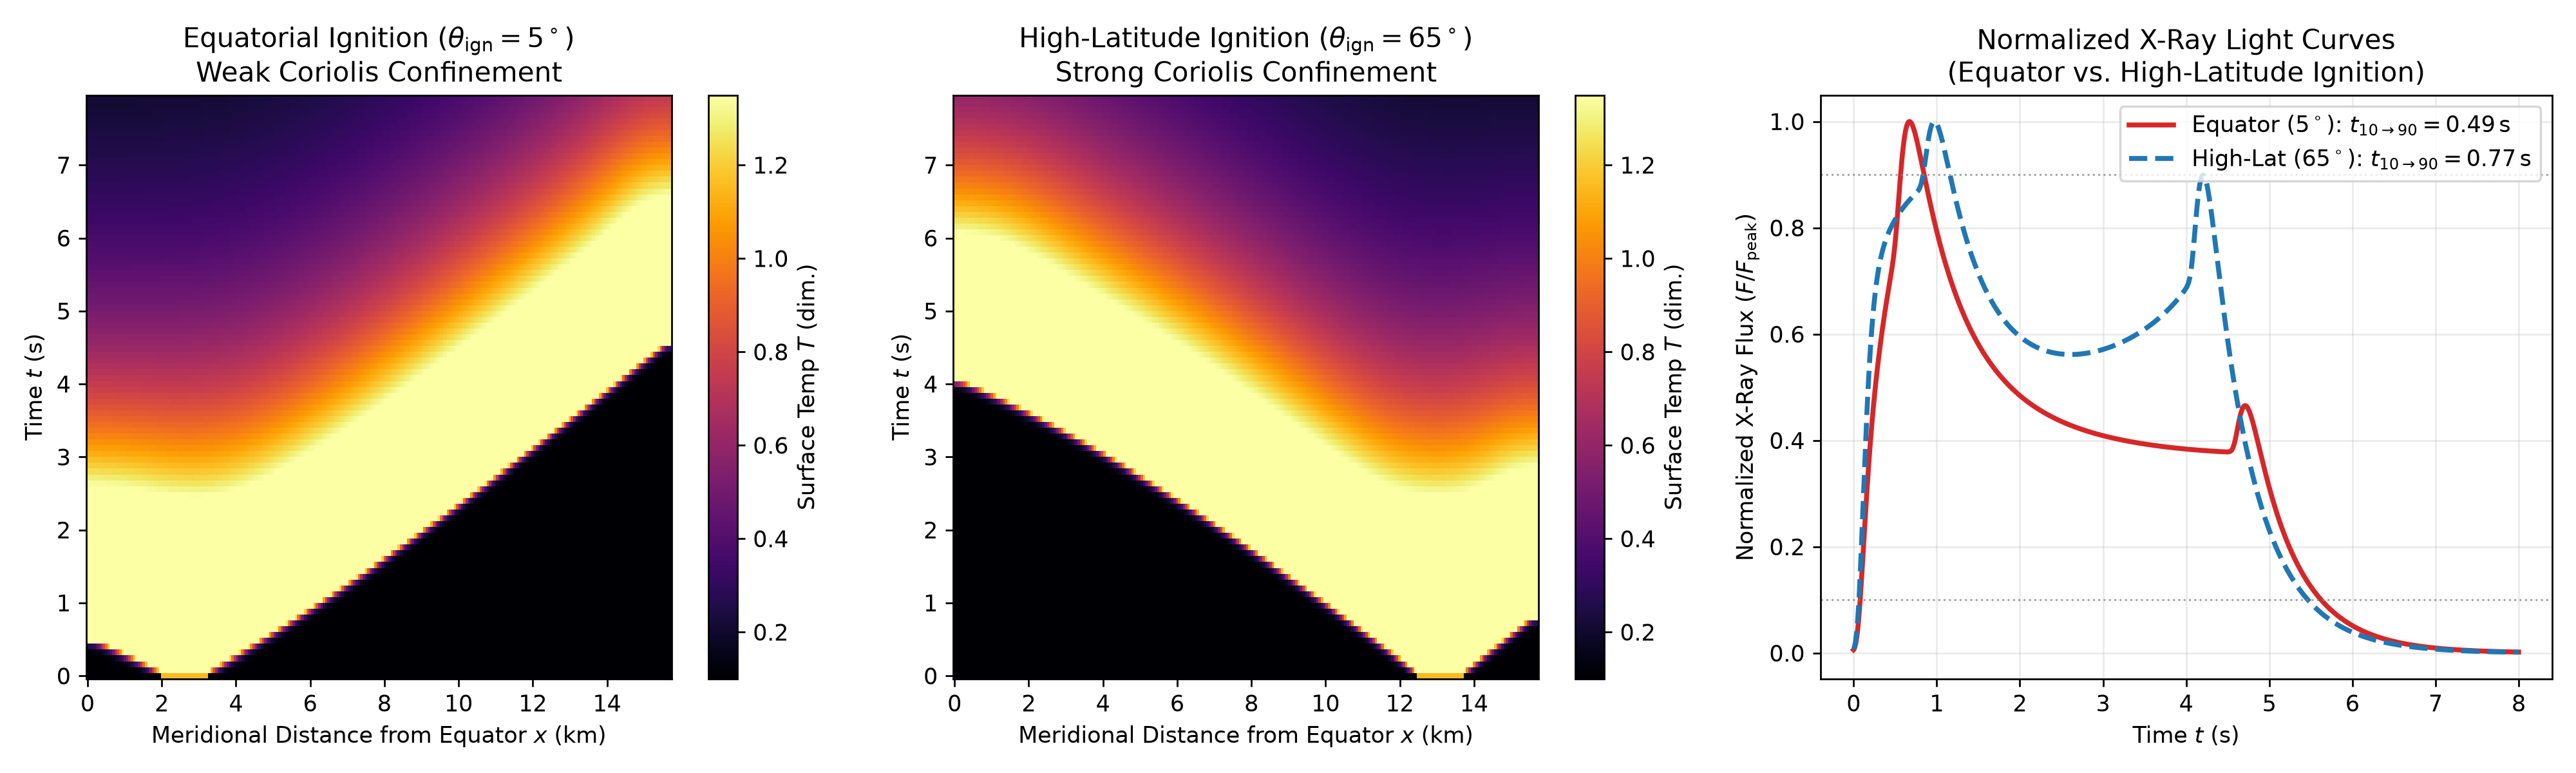
\includegraphics[width=\textwidth]{../outputs/equator_vs_high_latitude_comparison.png}
    \caption{Space-time temperature evolution for equatorial ignition ($\theta_{\mathrm{ign}} = 15^\circ$, left) versus high-latitude ignition ($\theta_{\mathrm{ign}} = 75^\circ$, center), alongside normalized disk-integrated X-ray light curves (right) showing the $t_{10 \to 90}$ rise-time divergence.}
    \label{fig:comparison}
\end{figure}

\subsection{Simulation Results}
Figure~\ref{fig:comparison} (generated in \texttt{outputs/}) compares the $15^\circ$ and $75^\circ$ simulations ($w_{\mathrm{ign}} = 1.2\,\mathrm{km}$, $\alpha = 2.5$). Under weak equatorial Coriolis confinement, the flame sweeps rapidly across the surface, producing a steep rise time ($t_{10 \to 90} \approx 1.3$--$1.6\,\mathrm{s}$). At $75^\circ$, on the other hand, Coriolis confinement suppresses polar diffusivity by $(1 + 2.5\sin 75^\circ) \approx 3.4\times$, slowing down front propagation and stretching the rise time ($t_{10 \to 90} \approx 3.8$--$4.5\,\mathrm{s}$), reproducing the bimodal fast and slow burst classes that were also observed in 4U~1730--22 by \citet{Bult2022}.

\subsection{The Interactive and Live API Dashboards}
The interactive dashboard helps to quickly test how the X-ray light curve changes when you vary parameters such as the ignition latitude. To provide this, \texttt{app.py} combines a Streamlit/Plotly interface with \texttt{src/heasarc\_client.py}:
\begin{itemize}
    \item \textbf{Interactive Simulation Tab (Parameter Sensitivity):} Sliders for ignition latitude ($0^\circ$--$85^\circ$), polar Coriolis drag ($\alpha \in [0, 4.5]$), and hotspot width ($0.4$--$2.5\,\mathrm{km}$) recompute the PDE solution on the fly, updating the 2D space-time heatmap, normalized X-ray light curve, CFL stability readout, and a live hotspot-quenching warning.
    \item \textbf{Live NASA HEASARC Observational Tab (Empirical Benchmarking):} \texttt{HeasarcBurstClient} queries NASA's HEASARC Virtual Observatory Table Access Protocol (\texttt{TAP/sync}) \citep{HEASARC_TAP} using Astronomical Data Query Language (ADQL) to fetch observed Type-I burst rise times (\texttt{trise}) and durations (\texttt{bdur}) from the MINBAR catalog \citep{Galloway2020} for sources such as \texttt{4U~1730-22} and \texttt{GS~1826-24} (falling back seamlessly to published benchmark values when offline). Overlaying the simulated $t_{10 \to 90}$ onto empirical burst rise-time histograms immediately shows which observational regime a parameter set reproduces.
\end{itemize}
\textbf{How to Run:} From the repository root, install dependencies (\texttt{pip install -r requirements.txt}) and launch \texttt{streamlit run app.py}.

\section{Limitations and Future Improvements}

While this 1D planar model captures the primary Coriolis rise-time dichotomy, three extensions would bring it closer to full astrophysical fidelity:
\begin{enumerate}
    \item \textbf{Spherical Metric Area Weighting:} Weighting each cell's flux contribution by $\cos\theta\,dx$ and incorporating the spherical convergence term away from the polar singularity will capture the smaller emitting area of polar caps relative to the equatorial belt.
    \item \textbf{2D Shallow-Water Magnetohydrodynamics:} Extending the spatial grid to latitude--longitude $(\theta, \phi)$ shallow-water equations \citep{Spitkovsky2002} will resolve azimuthal flame asymmetries responsible for coherent burst oscillations ($\sim 584.65\,\mathrm{Hz}$ in 4U~1730--22).
    \item \textbf{Multi-Step Nuclear Burning Networks:} Replacing single-step Arrhenius burning with coupled triple-$\alpha$ helium ignition and $rp$-process hydrogen capture via the \texttt{ReactionModel} interface will capture prolonged burst decay tails and instrument energy-band responses.
\end{enumerate}

\section{Conclusion}

By using a 1D reaction--diffusion PDE solver alongside an interactive parameter explorer dashboard \texttt{thermonuclear-ignition-sim-1d} demonstrates how ignition latitude and Coriolis confinement affect lateral flame propagation, which is directly reflected in the resulting X-ray light curve.

\bibliographystyle{plainnat}
\bibliography{references}

\end{document}
